% !TEX program = pdflatex
% ===========================================================================
% Enterprise Banking Risk Management Dashboard — Technical Documentation
% ===========================================================================
% Compile with:  pdflatex project-documentation-en.tex  (×2 for TOC)
% ===========================================================================

\documentclass[12pt,a4paper]{article}

% === Packages ===
\usepackage[utf8]{inputenc}
\usepackage[T1]{fontenc}
\usepackage{newtxtext,newtxmath}
\usepackage{graphicx}
\usepackage{float}
\usepackage{longtable}
\usepackage{booktabs}
\usepackage{hyperref}
\usepackage{enumitem}
\usepackage{fancyhdr}
\usepackage{geometry}
\usepackage{xcolor}
\usepackage{tikz}
\usepackage{listings}
\usetikzlibrary{shapes,arrows,positioning,fit,backgrounds}

\geometry{margin=2.5cm}
\hypersetup{
    colorlinks=true,
    linkcolor=blue!60!black,
    urlcolor=blue!50!black,
    citecolor=green!50!black,
}

% === Page Style ===
\pagestyle{fancy}
\fancyhf{}
\fancyhead[RO,LE]{\small Bank Risk Management Dashboard}
\fancyhead[LO,RE]{\small Technical Documentation}
\fancyfoot[C]{\thepage}
\renewcommand{\headrulewidth}{0.5pt}

% === Colors ===
\definecolor{lightblue}{RGB}{235,245,255}
\definecolor{lightgreen}{RGB}{235,255,240}
\definecolor{codebg}{RGB}{248,248,250}

% === Code Style ===
\lstset{
    basicstyle=\ttfamily\small,
    backgroundcolor=\color{codebg},
    frame=single,
    framerule=0.5pt,
    rulecolor=\color{gray!40},
    breaklines=true,
    showstringspaces=false,
    tabsize=2,
    aboveskip=8pt,
    belowskip=8pt,
}

% === Document ===
\begin{document}

% ===== TITLE PAGE =====
\begin{titlepage}
\begin{center}
\vspace*{2cm}

{\Huge\bfseries Enterprise Banking Risk\\[6pt] Management Dashboard}

\vspace{0.8cm}
{\LARGE AI-Enabled Risk Intelligence Platform}

\vspace{1.5cm}
{\large Technical Documentation \& User Guide}

\vspace{1cm}
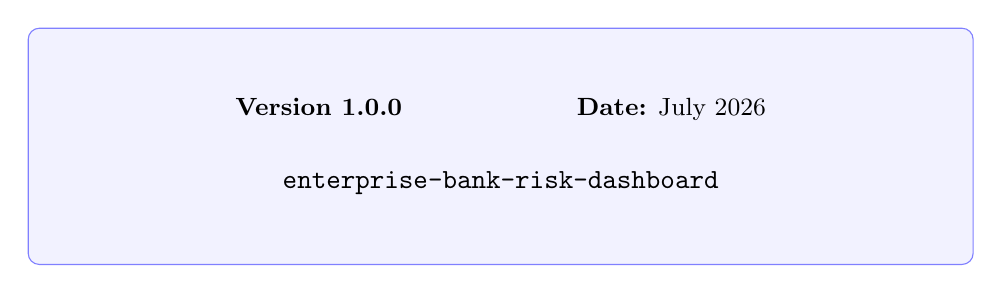
\begin{tikzpicture}
\node[draw=blue!50,fill=blue!5,rounded corners,inner sep=20pt,
      minimum width=12cm,minimum height=3cm] {
\begin{minipage}{10cm}
\begin{center}
{\small\textbf{Version 1.0.0} \hspace{2cm} \textbf{Date:} July 2026}

\vspace{0.5cm}
\texttt{enterprise-bank-risk-dashboard}
\end{center}
\end{minipage}
};
\end{tikzpicture}

\vspace{1.5cm}

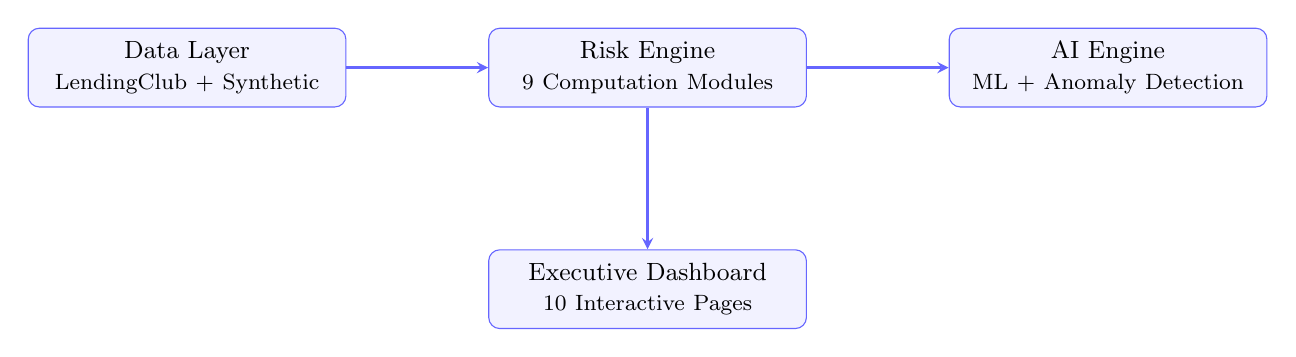
\begin{tikzpicture}[node distance=1.8cm,auto,
    block/.style={rectangle,draw=blue!60,fill=blue!5,rounded corners,
                  text width=3.8cm,align=center,minimum height=1cm,font=\small},
    arrow/.style={->,>=stealth,thick,blue!60}]
\node[block] (data) {Data Layer\\\footnotesize{LendingClub + Synthetic}};
\node[block,right=of data] (engine) {Risk Engine\\\footnotesize{9 Computation Modules}};
\node[block,right=of engine] (ai) {AI Engine\\\footnotesize{ML + Anomaly Detection}};
\node[block,below=of engine] (ui) {Executive Dashboard\\\footnotesize{10 Interactive Pages}};
\draw[arrow] (data) -- (engine);
\draw[arrow] (engine) -- (ai);
\draw[arrow] (engine) -- (ui);
\end{tikzpicture}

\vfill
{\small \textcopyright\ 2026 All Rights Reserved}
\end{center}
\end{titlepage}

% ===== TABLE OF CONTENTS =====
\newpage
\tableofcontents
\newpage

% ===================================================================
\section{Overview}
% ===================================================================

This platform provides a comprehensive risk management system for commercial banks, digital banks, and financial institutions. It combines traditional risk measurement with artificial intelligence, macroeconomic analysis, and predictive analytics.

\subsection{Coverage Domains}
\begin{enumerate}[itemsep=4pt]
    \item Credit Portfolio Risk
    \item Portfolio Concentration Risk
    \item Risk-Adjusted Performance
    \item Sector \& Market Conditions
    \item Macroeconomic Risk
    \item Liquidity \& Funding Risk
    \item Capital Adequacy Risk
    \item Stress Testing \& Scenario Analysis
    \item AI Early Warning \& Forecasting
\end{enumerate}

\subsection{Data Sources}
\begin{itemize}
    \item Real LendingClub loan data (2007--2018) --- 151 columns, 2.26M accepted + 27.6M rejected loans
    \item Synthetically generated market and macroeconomic data (when real data unavailable)
    \item User-uploadable CSV/Excel files via sidebar
\end{itemize}

% ===================================================================
\section{System Architecture}
% ===================================================================

The system follows a layered architecture where each layer has a distinct responsibility:

\begin{figure}[H]
\centering
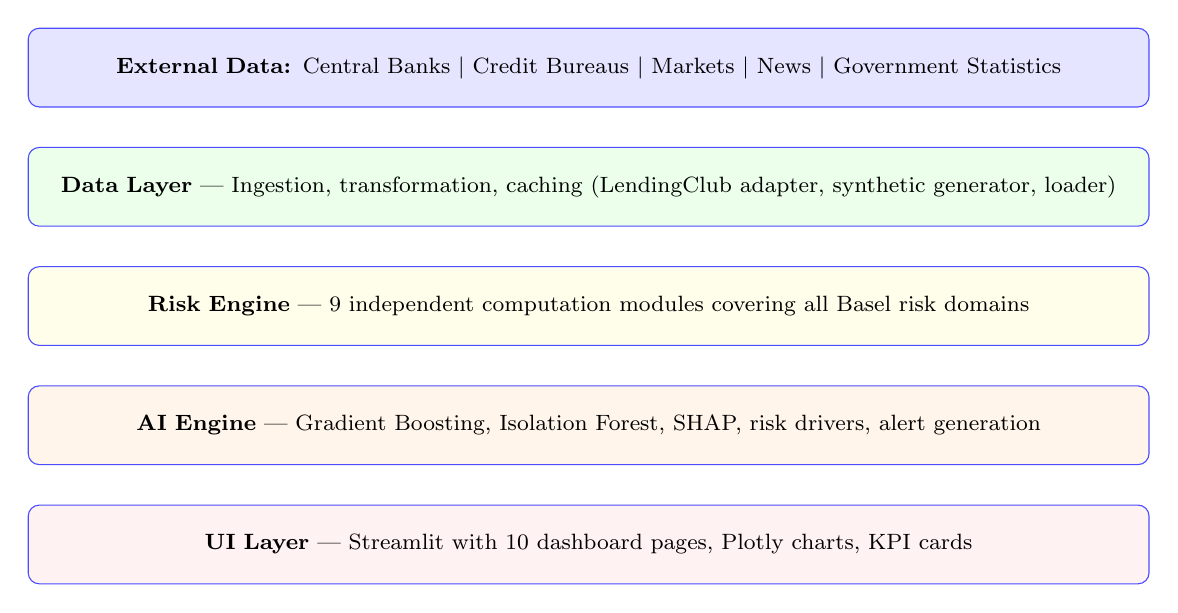
\begin{tikzpicture}[
    node distance=0.5cm,
    layer/.style={rectangle,draw=blue!70,fill=blue!3,rounded corners,
                  text width=14cm,align=center,minimum height=1cm,font=\footnotesize},
]
\node[layer,fill=blue!10] (l1) {\textbf{External Data:} Central Banks $|$ Credit Bureaus $|$ Markets $|$ News $|$ Government Statistics};
\node[layer,below=of l1,fill=green!8] (l2) {\textbf{Data Layer} — Ingestion, transformation, caching (LendingClub adapter, synthetic generator, loader)};
\node[layer,below=of l2,fill=yellow!8] (l3) {\textbf{Risk Engine} — 9 independent computation modules covering all Basel risk domains};
\node[layer,below=of l3,fill=orange!8] (l4) {\textbf{AI Engine} — Gradient Boosting, Isolation Forest, SHAP, risk drivers, alert generation};
\node[layer,below=of l4,fill=red!5] (l5) {\textbf{UI Layer} — Streamlit with 10 dashboard pages, Plotly charts, KPI cards};
\end{tikzpicture}
\caption{Layered System Architecture}
\end{figure}

\subsection{Project File Tree}

{\small
\begin{lstlisting}[language={},basicstyle=\ttfamily\scriptsize]
bank-risk/
├── app/                              # Streamlit UI
│   ├── main.py                       # Entry point + st.navigation sidebar
│   ├── components/
│   │   └── ui.py                     # KPI cards, chart builders, formatters
│   └── pages/
│       ├── executive_overview.py     # C-suite 360° view + risk heatmap
│       ├── credit_risk.py            # PD, EAD, LGD, ECL, NPL, vintage
│       ├── concentration_risk.py     # HHI, single-borrower, sector/geo treemaps
│       ├── risk_adjusted_performance.py  # RAROC, NIM, income waterfall
│       ├── sector_market.py          # Yield curve, FX, commodities, credit spreads
│       ├── macroeconomic.py          # GDP, CPI, unemployment, crisis probability
│       ├── liquidity_funding.py      # LCR gauge, NSFR, maturity ladder
│       ├── capital_adequacy.py       # CET1, CAR gauge, capital stack waterfall
│       ├── stress_testing.py         # 8 scenarios, ECL fan chart, reverse stress
│       └── ai_early_warning.py       # ML model, anomaly detection, feature importance
├── risk_engine/                      # Risk computation layer
│   ├── credit.py                     # PD, EAD, LGD, ECL, UL, NPL, vintage analysis
│   ├── concentration.py              # HHI, single-borrower, sector/geo, diversification
│   ├── performance.py                # RAROC, NIM, ROA, ROE, economic capital
│   ├── market.py                     # VaR (Hist/Param/MC), CVaR, drawdowns, volatility
│   ├── macro.py                      # Economic cycle, crisis probability, sensitivity
│   ├── liquidity.py                  # LCR, NSFR, maturity ladder, deposit concentration
│   ├── capital.py                    # CET1, Tier 1, CAR, leverage, capital buffer
│   ├── stress.py                     # 8 scenarios, reverse stress test
│   └── ai_models.py                  # GradientBoosting, IsolationForest, XAI drivers
├── data/
│   ├── lendingclub_adapter.py        # Maps 151 LendingClub columns → dashboard schema
│   ├── sample_generator.py           # Synthetic data generator (2000+ loans)
│   └── loader.py                     # Priority loader: LC > upload > synthetic
├── config/settings.py                # Bank config, sector/region/rating definitions
├── tests/test_smoke.py               # Integration smoke test
├── sample_data/                      # LendingClub CSVs (2 files, ~3.4 GB total)
├── requirements.txt
└── pyproject.toml
\end{lstlisting}
}

% ===================================================================
\section{Data Layer}
% ===================================================================

\subsection{Loading Priority}
Data is loaded in the following priority order:

\begin{enumerate}
    \item Session state cache (in-memory)
    \item LendingClub data from \texttt{sample\_data/} folder
    \item User-uploaded CSV/Excel file
    \item Auto-generated synthetic data (fallback)
\end{enumerate}

\subsection{LendingClub Column Mapping}

The 151-column LendingClub accepted loans CSV is mapped to the dashboard's expected schema:

\begin{longtable}{|>{\ttfamily\footnotesize}p{4.2cm}|>{\ttfamily\footnotesize}p{4.2cm}|p{4.5cm}|}
\caption{LendingClub to Dashboard Column Mapping}
\hline
\textbf{LendingClub Column} & \textbf{Dashboard Column} & \textbf{Notes} \\
\hline
\endfirsthead
\hline
\textbf{LendingClub Column} & \textbf{Dashboard Column} & \textbf{Notes} \\
\hline
\endhead
loan\_amnt / out\_prncp & original\_amount / outstanding\_balance & Loan amount \& remaining principal \\
int\_rate & interest\_rate & Parsed from string, divided by 100 \\
grade (A--G) & risk\_grade (AA--CC) & Mapped to internal Basel-aligned grades \\
purpose & sector & 12 industry categories \\
addr\_state & region & US state as geographic region \\
loan\_status & days\_past\_due, is\_npl, is\_defaulted & Status-derived flags \\
fico\_range\_low / fico\_range\_high & credit\_score & Averaged FICO score \\
annual\_inc & borrower\_income & Annual income, floored at 0 \\
recoveries & recovery\_amount & Dollar amount recovered post-default \\
term & term\_months & Parsed ``36 months'' $\rightarrow$ 36 \\
issue\_d & origination\_date & Parsed ``Dec-2014'' format \\
funded\_amnt & funded\_amount & Amount funded \\
hardship\_flag & is\_restructured & Y $\rightarrow$ True \\
\hline
\end{longtable}

\subsection{Derived Fields}

After mapping, the following are computed:

\begin{itemize}
    \item \textbf{PD:} Based on risk grade, mapped to standard Basel PD ranges (AAA=0.01\%, CC=22\%). Adjusted upward for already-delinquent loans.
    \item \textbf{LGD:} $1 - (\text{recoveries} / \text{original\_amount})$, floored at 0.30 (unsecured lending).
    \item \textbf{ECL:} $PD \times EAD \times LGD$
    \item \textbf{Unexpected Loss:} ECL multiplier based on PD standard deviation per grade.
\end{itemize}

% ===================================================================
\section{Risk Engine Layer}
% ===================================================================

Nine independent computation modules, each covering a specific risk domain.

\subsection{Credit Risk (\texttt{credit.py})}

\textbf{Core Metrics:}
\begin{center}
\begin{tabular}{|l|c|l|}
\hline
\textbf{Metric} & \textbf{Formula} & \textbf{Description} \\
\hline
Probability of Default (PD) & -- & Avg / EAD-weighted PD across portfolio \\
Exposure at Default (EAD) & Outstanding + Committed Undrawn & Total exposure when default occurs \\
Loss Given Default (LGD) & 1 − (Recovery / EAD) & Loss severity \\
Expected Credit Loss (ECL) & PD $\times$ EAD $\times$ LGD & Expected future losses \\
Unexpected Loss (UL) & ECL $\times$ multiplier & 99.9\% confidence tail loss \\
NPL Ratio & NPL Balance / Total Loans & Portfolio deterioration \\
Default Rate & Defaulted Loans / Total Loans & Credit quality \\
Recovery Rate & Recovered / Defaulted EAD & Recovery effectiveness \\
Write-off Rate, Restructuring Rate & -- & Permanent loss \& borrower stress \\
\hline
\end{tabular}
\end{center}

Additional outputs: PD distribution by grade, ECL by sector, vintage analysis (NPL by origination year), delinquency funnel.

\subsection{Concentration Risk (\texttt{concentration.py})}

\begin{itemize}
    \item \textbf{HHI (Borrower):} $\sum (\text{exposure\_share}_i)^2$
    \item \textbf{HHI (Sector), HHI (Region):} Same formula per dimension
    \item \textbf{Single Borrower Ratio:} Largest exposure / Total capital
    \item \textbf{Top-10 / Top-20 Ratio:} Share of 10/20 largest exposures
    \item \textbf{Diversification Benefit:} $1 - \sqrt{\text{HHI}}$
    \item \textbf{Related Party Ratio:} Related-party exposure / Capital
\end{itemize}

\subsection{Risk-Adjusted Performance (\texttt{performance.py})}

\begin{itemize}
    \item \textbf{RAROC:} (Interest Income $-$ Interest Expense $-$ Op. Cost $-$ Credit Losses) / Economic Capital
    \item \textbf{NIM:} (Interest Income $-$ Interest Expense) / Earning Assets
    \item \textbf{ROA:} Net Income / Total Assets
    \item \textbf{ROE:} Net Income / Shareholder Equity
    \item \textbf{Cost of Credit Risk:} Credit Losses / Average Loans
\end{itemize}

Outputs an income statement waterfall: Interest Income $\rightarrow$ Net Interest Income $\rightarrow$ Pre-Provision Profit $\rightarrow$ Post-Provision Profit.

\subsection{Market Risk (\texttt{market.py})}

\begin{itemize}
    \item \textbf{VaR (3 methods):} Historical, Parametric (normal), Monte Carlo simulation
    \item \textbf{Expected Shortfall (CVaR):} Average loss beyond VaR threshold
    \item \textbf{Maximum Drawdown:} Peak-to-trough decline
    \item \textbf{Annualized Volatility:} $\sigma \times \sqrt{12}$
    \item \textbf{Market Indicators:} Policy rate, yield spread, credit spreads, FX, commodities, housing, PMI, consumer confidence
\end{itemize}

\subsection{Macroeconomic Risk (\texttt{macro.py})}

\begin{itemize}
    \item \textbf{Economic Cycle Classification:} Expansion (>2.5\% GDP) / Recovery (>1\%) / Slowdown / Recession (<-1\%)
    \item \textbf{Crisis Probability:} Heuristic scoring from GDP, unemployment, inflation, government debt
    \item \textbf{Portfolio Sensitivity:} NPL elasticity to GDP ($\beta \approx -0.35$) and unemployment ($\beta \approx 0.25$)
\end{itemize}

\subsection{Liquidity Risk (\texttt{liquidity.py})}

\begin{itemize}
    \item \textbf{LCR:} HQLA / Net Cash Outflows (30-day)
    \item \textbf{NSFR:} Available Stable Funding / Required Stable Funding
    \item \textbf{Liquidity Gap:} HQLA $-$ Net Outflows
    \item \textbf{Deposit Concentration:} Top-10 deposits / Total deposits
    \item \textbf{Maturity Ladder:} Assets vs liabilities by time bucket
\end{itemize}

\subsection{Capital Adequacy (\texttt{capital.py})}

\begin{itemize}
    \item \textbf{CET1 Ratio:} Core Capital / RWA
    \item \textbf{Tier 1 Ratio:} (CET1 + AT1) / RWA
    \item \textbf{Total CAR:} Total Capital / RWA
    \item \textbf{Leverage Ratio:} Tier 1 / Total Exposure
    \item \textbf{Capital Buffer:} Available capital $-$ Required capital (incl. conservation buffer)
\end{itemize}

\subsection{Stress Testing (\texttt{stress.py})}

\textbf{Eight predefined scenarios:}

\begin{enumerate}[itemsep=2pt]
    \item \textbf{Baseline} --- no shock
    \item \textbf{Economic Recession} --- GDP $-4\%$, unemployment $+4\%$
    \item \textbf{Interest Rate Shock} --- rates $+300$ bps, housing $-15\%$
    \item \textbf{Inflation Shock} --- CPI $+5\%$, rates $+200$ bps
    \item \textbf{Currency Crisis} --- FX depreciation $30\%$, rates $+400$ bps
    \item \textbf{Commodity Price Collapse} --- commodities $-40\%$
    \item \textbf{Housing Market Crisis} --- housing $-30\%$, GDP $-3.5\%$
    \item \textbf{Severe Combined Shock} --- all shocks simultaneously
\end{enumerate}

Each scenario computes: stressed NPL ratio, stressed ECL, stressed CAR, capital shortfall.

\textbf{Reverse Stress Test:} Computes the NPL ratio, GDP decline, and unemployment rate that would push CAR below the regulatory minimum.

\subsection{AI Models (\texttt{ai\_models.py})}

\begin{itemize}
    \item \textbf{Default Prediction:} \texttt{GradientBoostingClassifier} trained on 6 features (balance, rate, term, collateral, income, credit score). Reports AUC, precision, recall, F1.
    \item \textbf{Anomaly Detection:} \texttt{IsolationForest} with 5\% contamination --- flags anomalous loans.
    \item \textbf{Risk Drivers (XAI):} Top-10 features ranked by absolute correlation with NPL status. Falls back to SHAP when available.
    \item \textbf{Alert Generation:} Rule-based + AI alerts: NPL threshold breach, anomaly count, sector NPL outlier, model AUC degradation.
\end{itemize}

% ===================================================================
\section{User Interface Layer}
% ===================================================================

The UI is built with \textbf{Streamlit} using \texttt{st.navigation} for sidebar-based page switching. All charts use \textbf{Plotly} for interactivity.

\subsection{Page 1: Executive Overview}

\begin{itemize}
    \item 6 KPI cards: ECL, NPL Ratio, CAR, LCR, RAROC, AI Alerts
    \item Risk heatmap: 6 domains $\times$ 2 dimensions (current, outlook)
    \item 12-month ECL \& NPL trend simulation
    \item AI early warning alert feed with color-coded severity
    \item Top-10 risk exposures table
    \item Regulatory headroom table (CET1, Tier1, CAR, Leverage, LCR, NSFR)
\end{itemize}

\subsection{Page 2: Credit Portfolio Risk}

\begin{itemize}
    \item PD / LGD / EAD / ECL / UL KPI cards (simple and weighted averages)
    \item NPL, Default, Recovery, Write-off, Restructuring rates
    \item Delinquency funnel: 30+ $\rightarrow$ 60+ $\rightarrow$ 90+ DPD
    \item PD distribution bar chart by internal risk grade
    \item Vintage analysis: NPL rate by origination year
    \item ECL by sector (horizontal bar)
    \item High-risk loan watchlist (top 20 by PD)
\end{itemize}

\subsection{Page 3: Portfolio Concentration}

\begin{itemize}
    \item HHI (Borrower, Sector), Single Borrower / Capital, Top-10 share
    \item Treemap: exposure by sector, colored by NPL ratio
    \item Horizontal bar: top-20 borrower exposures
    \item Donut chart: geographic concentration by region
    \item Regulatory guideline compliance table
\end{itemize}

\subsection{Page 4: Risk-Adjusted Performance}

\begin{itemize}
    \item RAROC, NIM, ROA, ROE, Cost of Credit KPI cards
    \item Income statement waterfall chart
    \item Performance ratios with industry benchmarks
    \item Economic capital vs ECL vs Risk-Adjusted Income
\end{itemize}

\subsection{Page 5: Sector \& Market Conditions}

\begin{itemize}
    \item Policy rate, 10Y-2Y spread, credit spreads (AAA/BBB/HY)
    \item FX rate, FX volatility, commodity index, oil price, housing index
    \item Yield curve comparison: current vs 3 months ago
    \item Credit spreads time series
    \item PMI, consumer confidence, housing YoY
    \item Indexed 12-month market overview
\end{itemize}

\subsection{Page 6: Macroeconomic Risk}

\begin{itemize}
    \item GDP growth, CPI, unemployment, government debt/GDP, fiscal balance
    \item Economic cycle phase indicator
    \item Crisis probability gauge (0--100\%, color-coded thresholds)
    \item Portfolio macro sensitivity table (GDP $\beta$, unemployment $\beta$)
    \item GDP vs Inflation trend, Unemployment vs Debt trend (dual-axis)
\end{itemize}

\subsection{Page 7: Liquidity \& Funding}

\begin{itemize}
    \item LCR gauge (50--200\%, with 100\% threshold)
    \item NSFR, liquidity gap, deposit concentration, funding cost
    \item Deposit segment breakdown donut chart
    \item Maturity ladder: assets vs liabilities by bucket with cumulative gap
    \item Top-10 depositor concentration table
\end{itemize}

\subsection{Page 8: Capital Adequacy}

\begin{itemize}
    \item CET1, Tier 1, Total CAR, Leverage Ratio, RWA Density
    \item Capital stack waterfall: CET1 $\rightarrow$ +AT1 $\rightarrow$ Tier 1 $\rightarrow$ +T2 $\rightarrow$ Total
    \item CAR gauge vs regulatory minimum
    \item RWA composition donut (Credit 75\% / Market 15\% / Operational 10\%)
    \item Capital buffer breakdown bar chart
\end{itemize}

\subsection{Page 9: Stress Testing}

\begin{itemize}
    \item Scenario selector dropdown (8 scenarios)
    \item Shock parameter display (GDP, Rate, Unemployment, Housing)
    \item Stressed NPL, Stressed ECL, Stressed CAR, Capital Shortfall cards
    \item NPL increase comparison bar chart (all scenarios)
    \item CAR impact comparison bar chart (all scenarios)
    \item ECL trajectory fan chart (5-year horizon, 5 scenarios)
    \item Reverse stress test: break NPL, break GDP, break unemployment
    \item Detailed scenario results table
\end{itemize}

\subsection{Page 10: AI Early Warning}

\begin{itemize}
    \item Alert summary: Critical / Warning / Watch counts
    \item Color-coded alert feed with domain tags
    \item Model performance cards: AUC, Precision, Recall, F1, sample count
    \item Feature importance bar chart (from Gradient Boosting)
    \item Top-10 risk drivers (correlation with NPL)
    \item Anomaly scatter plot: PD vs Balance, flagged in red
    \item AI-predicted PD vs Original PD comparison by grade
\end{itemize}

% ===================================================================
\section{Open Source Technology Stack}
% ===================================================================

\begin{longtable}{|p{3.5cm}|p{3.8cm}|p{5.5cm}|}
\caption{Open Source Technologies Used}
\hline
\textbf{Domain} & \textbf{Technology} & \textbf{Repository} \\
\hline
\endfirsthead
\hline
\textbf{Domain} & \textbf{Technology} & \textbf{Repository} \\
\hline
\endhead

Dashboard \& UI & Streamlit & \texttt{github.com/streamlit/streamlit} \\
Charts & Plotly & \texttt{github.com/plotly/plotly.py} \\
Data Processing & Pandas, NumPy & \texttt{github.com/pandas-dev/pandas} \\
Machine Learning & scikit-learn & \texttt{github.com/scikit-learn/scikit-learn} \\
Anomaly Detection & Isolation Forest & (scikit-learn built-in) \\
Gradient Boosting & GradientBoostingClassifier & (scikit-learn built-in) \\
Statistics & SciPy & \texttt{github.com/scipy/scipy} \\
Explainable AI & SHAP & \texttt{github.com/shap/shap} \\
Configuration & PyYAML & \texttt{github.com/yaml/pyyaml} \\
Excel Support & openpyxl & \texttt{github.com/tox-dev/openpyxl} \\
Environment & python-dotenv & \texttt{github.com/theskumar/python-dotenv} \\
\hline
\end{longtable}

% ===================================================================
\section{Installation \& Usage}
% ===================================================================

\subsection{Prerequisites}
\begin{itemize}
    \item Python 3.10 or higher
    \item \texttt{pip} package manager
\end{itemize}

\subsection{Installation}

\begin{lstlisting}[language=bash]
cd bank-risk/
pip install -r requirements.txt
\end{lstlisting}

\subsection{Running the Dashboard}

\begin{lstlisting}[language=bash]
PYTHONPATH=. streamlit run app/main.py
\end{lstlisting}

The dashboard is accessible at \texttt{http://localhost:8501}.

\subsection{Uploading Custom Data}

Via the sidebar panel under ``Data Management'' $\rightarrow$ upload a CSV or Excel file.

Expected columns: \texttt{outstanding\_balance}, \texttt{sector}, \texttt{region}, \texttt{risk\_grade}, \texttt{days\_past\_due}, \texttt{collateral\_value}, etc. Unrecognized columns are ignored gracefully.

\subsection{Switching Between Data Sources}

\begin{itemize}
    \item \textbf{Default:} LendingClub data from \texttt{sample\_data/} (50,000 loan sample)
    \item \textbf{User upload:} Sidebar upload overrides all other sources
    \item \textbf{Regenerate:} ``Reload Portfolio Data'' button reloads from LendingClub (or falls back to synthetic)
\end{itemize}

% ===================================================================
\section{Risk Metrics \& Formulas Summary}
% ===================================================================

\subsection{Credit Risk}
\begin{align*}
\text{ECL} &= PD \times EAD \times LGD \\
\text{NPL Ratio} &= \frac{\text{NPL Balance}}{\text{Total Loans}} \\
\text{Recovery Rate} &= \frac{\text{Recovered Amount}}{\text{Defaulted EAD}}
\end{align*}

\subsection{Concentration Risk}
\begin{align*}
\text{HHI} &= \sum_{i=1}^{n} (\text{exposure\_share}_i)^2 \\
\text{Diversification Benefit} &= 1 - \sqrt{\text{HHI}_{\text{borrower}}}
\end{align*}

\subsection{Risk-Adjusted Performance}
\begin{align*}
\text{RAROC} &= \frac{\text{Risk-Adjusted Income}}{\text{Economic Capital}} \\
\text{NIM} &= \frac{\text{Interest Income} - \text{Interest Expense}}{\text{Earning Assets}}
\end{align*}

\subsection{Market Risk}
\begin{align*}
\text{VaR}_{\alpha} &= \text{Percentile}(\text{returns}, 1-\alpha) \quad \text{(Historical)} \\
\text{VaR}_{\alpha} &= \mu + \sigma \cdot \Phi^{-1}(1-\alpha) \quad \text{(Parametric)} \\
\text{ES}_{\alpha} &= \mathbb{E}[\text{returns} \mid \text{returns} \leq \text{VaR}_{\alpha}]
\end{align*}

\subsection{Liquidity}
\begin{align*}
\text{LCR} &= \frac{\text{HQLA}}{\text{Net Cash Outflows}_{30\text{d}}} \\
\text{NSFR} &= \frac{\text{Available Stable Funding}}{\text{Required Stable Funding}}
\end{align*}

\subsection{Capital Adequacy}
\begin{align*}
\text{CET1 Ratio} &= \frac{\text{Core Capital}}{\text{RWA}} \\
\text{Total CAR} &= \frac{\text{Tier 1} + \text{Tier 2}}{\text{RWA}} \\
\text{Leverage Ratio} &= \frac{\text{Tier 1 Capital}}{\text{Total Exposure}}
\end{align*}

\subsection{Stress Test — NPL Elasticities}
\begin{align*}
\Delta\text{NPL} &= \varepsilon_{\text{GDP}} \cdot \Delta\text{GDP} \cdot \text{NPL}_{\text{base}}
                  + \varepsilon_{\text{rate}} \cdot \Delta\text{Rate} \cdot \text{NPL}_{\text{base}} \\
                &\quad + \varepsilon_{\text{unemp}} \cdot \Delta\text{Unemployment} \cdot \text{NPL}_{\text{base}} \\
                &\quad + \varepsilon_{\text{housing}} \cdot \Delta\text{Housing} \cdot \text{NPL}_{\text{base}}
\end{align*}
where $\varepsilon_{\text{GDP}} = -2.0$, $\varepsilon_{\text{rate}} = 0.08$, $\varepsilon_{\text{unemp}} = 1.5$, $\varepsilon_{\text{housing}} = 0.3$.

% ===================================================================
\section{Conclusion}
% ===================================================================

This platform delivers a comprehensive, integrated banking risk management solution:

\begin{itemize}[itemsep=3pt]
    \item \textbf{9 risk domains} aligned with Basel Committee requirements
    \item \textbf{Real loan data} from LendingClub with plug-and-play replacement
    \item \textbf{Computation engine} implementing industry-standard banking formulas
    \item \textbf{Artificial intelligence} for prediction, anomaly detection, and explainable risk drivers
    \item \textbf{Stress testing} with 8 predefined scenarios plus reverse stress analysis
    \item \textbf{Interactive UI} with dynamic Plotly charts and KPI cards
    \item \textbf{Modular architecture} enabling easy extension and maintenance
\end{itemize}

The layered, modular architecture allows any component to be replaced without affecting others — critical for institutions requiring customized risk models or data sources.

\vspace{1cm}
\begin{center}
{\Large\bfseries --- End of Document ---}
\end{center}

\end{document}
